% LaTeX Präsentationsvorlage (2013) der TU Graz, rev12, 2013/01/31
% !TeX encoding = UTF-8
\documentclass{beamer}
% \documentclass[aspectratio=169]{beamer}
% \usetheme{tugraz2013}
% \usetheme[notes]{tugraz2013}
\usepackage{../common/beamerthemetugraz2013}
\usepackage{color}
\usepackage{multicol}
\usepackage{bbding}
\usepackage{wasysym}
\usepackage{caption}
\usepackage{array}
% \usepackage{minted}

\usepackage{listings}
\usepackage{xcolor}

\definecolor{codegreen}{rgb}{0,0.6,0}
\definecolor{codegray}{rgb}{0.5,0.5,0.5}
\definecolor{codepurple}{rgb}{0.58,0,0.82}
\definecolor{backcolour}{rgb}{0.95,0.95,0.92}
\lstdefinestyle{mystyle}{
    backgroundcolor=\color{backcolour},   
    commentstyle=\color{codegreen},
    keywordstyle=\color{magenta},
    numberstyle=\tiny\color{codegray},
    stringstyle=\color{codepurple},
    basicstyle=\ttfamily\footnotesize,
    breakatwhitespace=false,         
    breaklines=true,                 
    captionpos=b,                    
    keepspaces=true,                 
    numbers=left,                    
    numbersep=5pt,                  
    showspaces=false,                
    showstringspaces=false,
    showtabs=false,                  
    tabsize=2
}

\lstset{style=mystyle}

\usepackage{picture}
\usepackage{rotating}
\definecolor{darkred}{rgb}{0.85,0.16,0.0}
\definecolor{darkgreen}{rgb}{0.16,0.70,0.27}

\usepackage{xcolor}


\newcommand{\hrefu}[2]{\underline{\href{#1}{#2}}}
\newcommand{\hyperlinku}[2]{\underline{\hyperlink{#1}{#2}}}
\newcommand{\smallurl}[1]{%
  \begin{flushleft}
    \tiny\url{#1}
  \end{flushleft}
}
\newcommand{\smalltext}[1]{%
  \begin{flushleft}
    \tiny{#1}
  \end{flushleft}
}
\newcommand{\red}[1]{{\color{red} #1}}
\newcommand{\blue}[1]{{\color{blue} #1}}
\newcommand{\darkgreen}[1]{\textcolor{darkgreen}{#1}}
\newcommand{\darkred}[1]{\textcolor{darkred}{#1}}

\newcommand*{\vpointer}{\vcenter{\hbox{\scalebox{1.5}{\large\pointer}}}}

\newcommand{\be}[1]{\begin{equation} \label{#1}}
\newcommand{\ee}{\end{equation}}
\newcommand{\bea}[1]{\begin{eqnarray} \label{#1}}
\newcommand{\eea}{\end{eqnarray}}
\newcommand{\bean}{\begin{eqnarray*}}
\newcommand{\eean}{\end{eqnarray*}}

\newcommand{\non}{\nonumber\\}
\newcommand{\eq}[1]{(\ref{#1})}
\newcommand{\difp}[2]{\frac{\partial #1}{\partial #2}}
\newcommand{\br}{{\bf r}}
\newcommand{\bR}{{\bf R}}
\newcommand{\bA}{{\bf A}}
\newcommand{\bB}{{\bf B}}
\newcommand{\bE}{{\bf E}}
\newcommand{\bm}{{\bf m}}
%\renewcommand{\bm}{{\bf m}}
\newcommand{\bn}{{\bf n}}
\newcommand{\bN}{{\bf N}}
\newcommand{\bp}{{\bf p}}
\newcommand{\bP}{{\bf P}}
\newcommand{\bF}{{\bf F}}
\newcommand{\by}{{\bf y}}
\newcommand{\bz}{{\bf z}}
\newcommand{\bZ}{{\bf Z}}
\newcommand{\bV}{{\bf V}}
\newcommand{\bv}{{\bf v}}
\newcommand{\bu}{{\bf u}}
\newcommand{\bx}{{\bf x}}
\newcommand{\bX}{{\bf X}}
\newcommand{\bW}{{\bf W}}
\newcommand{\bJ}{{\bf J}}
\newcommand{\bj}{{\bf j}}
\newcommand{\bk}{{\bf k}}
\newcommand{\bTheta}{{\bf \Theta}}
\newcommand{\btheta}{{\boldsymbol\theta}}
\newcommand{\bOmega}{{\bf \Omega}}
\newcommand{\bomega}{{\boldsymbol\omega}}
\newcommand{\brho}{{\boldsymbol\rho}}
\newcommand{\rd}{{\rm d}}
\newcommand{\rJ}{{\rm J}}
\newcommand{\ph}{{\varphi}}
\newcommand{\te}{\theta}
\newcommand{\tht}{\vartheta}
\newcommand{\vpar}{v_\parallel}
\newcommand{\vparkb}{v_{\parallel k b}}
\newcommand{\vparkm}{v_{\parallel k m}}
\newcommand{\Jpar}{J_\parallel}
\newcommand{\ppar}{p_\parallel}
\newcommand{\Bpstar}{B_\parallel^*}
\newcommand{\intpi}{\int\limits_{0}^{2\pi}}
\newcommand{\summ}{\sum \limits_{m=-\infty}^\infty}
\newcommand{\tb}{\tau_b(\uv)}
\newcommand{\bh}{{\bf h}}
\newcommand{\cE}{{\cal E}}
\newcommand{\bsigma}{{\boldsymbol\sigma}}
\newcommand{\bS}{{\mathbf S}}
\newcommand{\bI}{{\mathbf I}}
\newcommand{\odtwo}[2]{\frac{\rd #1}{\rd #2}}
\newcommand{\pdone}[1]{\frac{\partial}{\partial #1}}
\newcommand{\pdtwo}[2]{\frac{\partial #1}{\partial #2}}
\newcommand{\ds}{\displaystyle} % commands


%% Titelblatt-Einstellungen
\title[]
{Python 10}
\author[E.~Wachmann]{\scriptsize Elias Wachmann
}
\date{2024} % \today für heutiges Datum verwenden
\institute[Institute of Theoretical and Computational Physics]
{
}
\instituteurl{www.tugraz.at}
% \institutelogo{kurz.pdf}
%~ \additionallogo{merged_logos}
\AtBeginSection[]{
  \begin{frame}
  \vfill
  \centering
  \begin{beamercolorbox}[sep=8pt,center,shadow=true,rounded=true]{title}
    \usebeamerfont{title}\insertsectionhead\par%
  \end{beamercolorbox}
  \vfill
  \end{frame}
}
\lstset{
    literate={Ö}{{\"O}}1
             {Ä}{{\"A}}1
             {Ü}{{\"U}}1
             {ß}{{\ss}}1
             {ü}{{\"u}}1
             {ä}{{\"a}}1
             {ö}{{\"o}}1
}

%%%%%%%%%%%%%%%%%%%%%%%%%%%%%%%%%%%%%%%%%%%%%%%%%%%%%%%%%%%%%%%%%%%%%%%%%%%%
\begin{document}
%%%%%%%%%%%%%%%%%%%%%%%%%%%%%%%%%%%%%%%%%%%%%%%%%%%%%%%%%%%%%%%%%%%%%%%%%%%%
\titleframe

%\begin{frame}
%  \frametitle{Outline}
%  \tableofcontents%[hideallsubsections] 
%  \note{
%  	Meine Präsentation ist wie folgt strukturiert \ldots
%  }
%\end{frame}

\section*{Content}

\begin{frame}
\frametitle{Content}
  \tableofcontents
\end{frame}

%%%%%%%%%%%%%%%%%%%%%%%%%%%%%%%%%%%%%%%%%%%%%%%%%%%%%%%%%%%%%%%%%%%%%%%%%%%%

\section{Differentiation in Python}
\begin{frame}
    \frametitle{Numpy \texttt{numpy.gradient}}
    The \texttt{numpy.gradient} function calculates the gradient of an array using finite differences.
    \hrefu{https://numpy.org/doc/stable/reference/generated/numpy.gradient.html}{\texttt{numpy.gradient}}
    \begin{align}
        \label{eq:gradient}
      \frac{\partial f}{\partial x} \approx \frac{f(x + h) - f(x - h)}{2h}
    \end{align}
    where \( h \) is a small step size. For a one-dimensional array \( y \) with spacing \( dx \), the gradient is calculated as:
    \begin{align}
      \text{gradient}[\text{i}] = \frac{y[\text{i}+1] - y[\text{i}-1]}{2 \cdot dx}
    \end{align}
\end{frame}

\begin{frame}
  \frametitle{Numpy \texttt{numpy.gradient} Example}
  \lstinputlisting[language=python]{examples/gradient_example.py}
\end{frame}

\begin{frame}
  \frametitle{Scipy \texttt{scipy.misc.derivative}}
  The \texttt{scipy.misc.derivative} function calculates the numerical derivative of a function.
  \hrefu{https://docs.scipy.org/doc/scipy/reference/generated/scipy.misc.derivative.html}{\texttt{scipy.misc.derivative}}
  This function uses the central difference formula:
  see Equation \ref{eq:gradient} or \hrefu{https://en.wikipedia.org/wiki/Finite_difference}{Finite difference}
  \lstinputlisting[language=python]{examples/derivative_example.py}
\end{frame}

\section{Integration in Python}
\begin{frame}
  \frametitle{Scipy \texttt{scipy.integrate.trapezoid}}
  The \texttt{scipy.integrate.trapezoid} function computes the trapezoidal rule to approximate the integral.
  \hrefu{https://docs.scipy.org/doc/scipy/reference/generated/scipy.integrate.trapezoid.html}{\texttt{scipy.trapezoid}}
  \vspace{5mm}
  It uses the following approximate formula:
    \begin{align*}
        \int_{a}^{b} f(x) \, dx \approx \frac{b - a}{2} \left( f(a) + f(b) \right)
    \end{align*}
\end{frame}
\begin{frame}
    \frametitle{Intuition behind the Trapezoid Rule}
    \vspace{-5mm}
    \begin{center}
        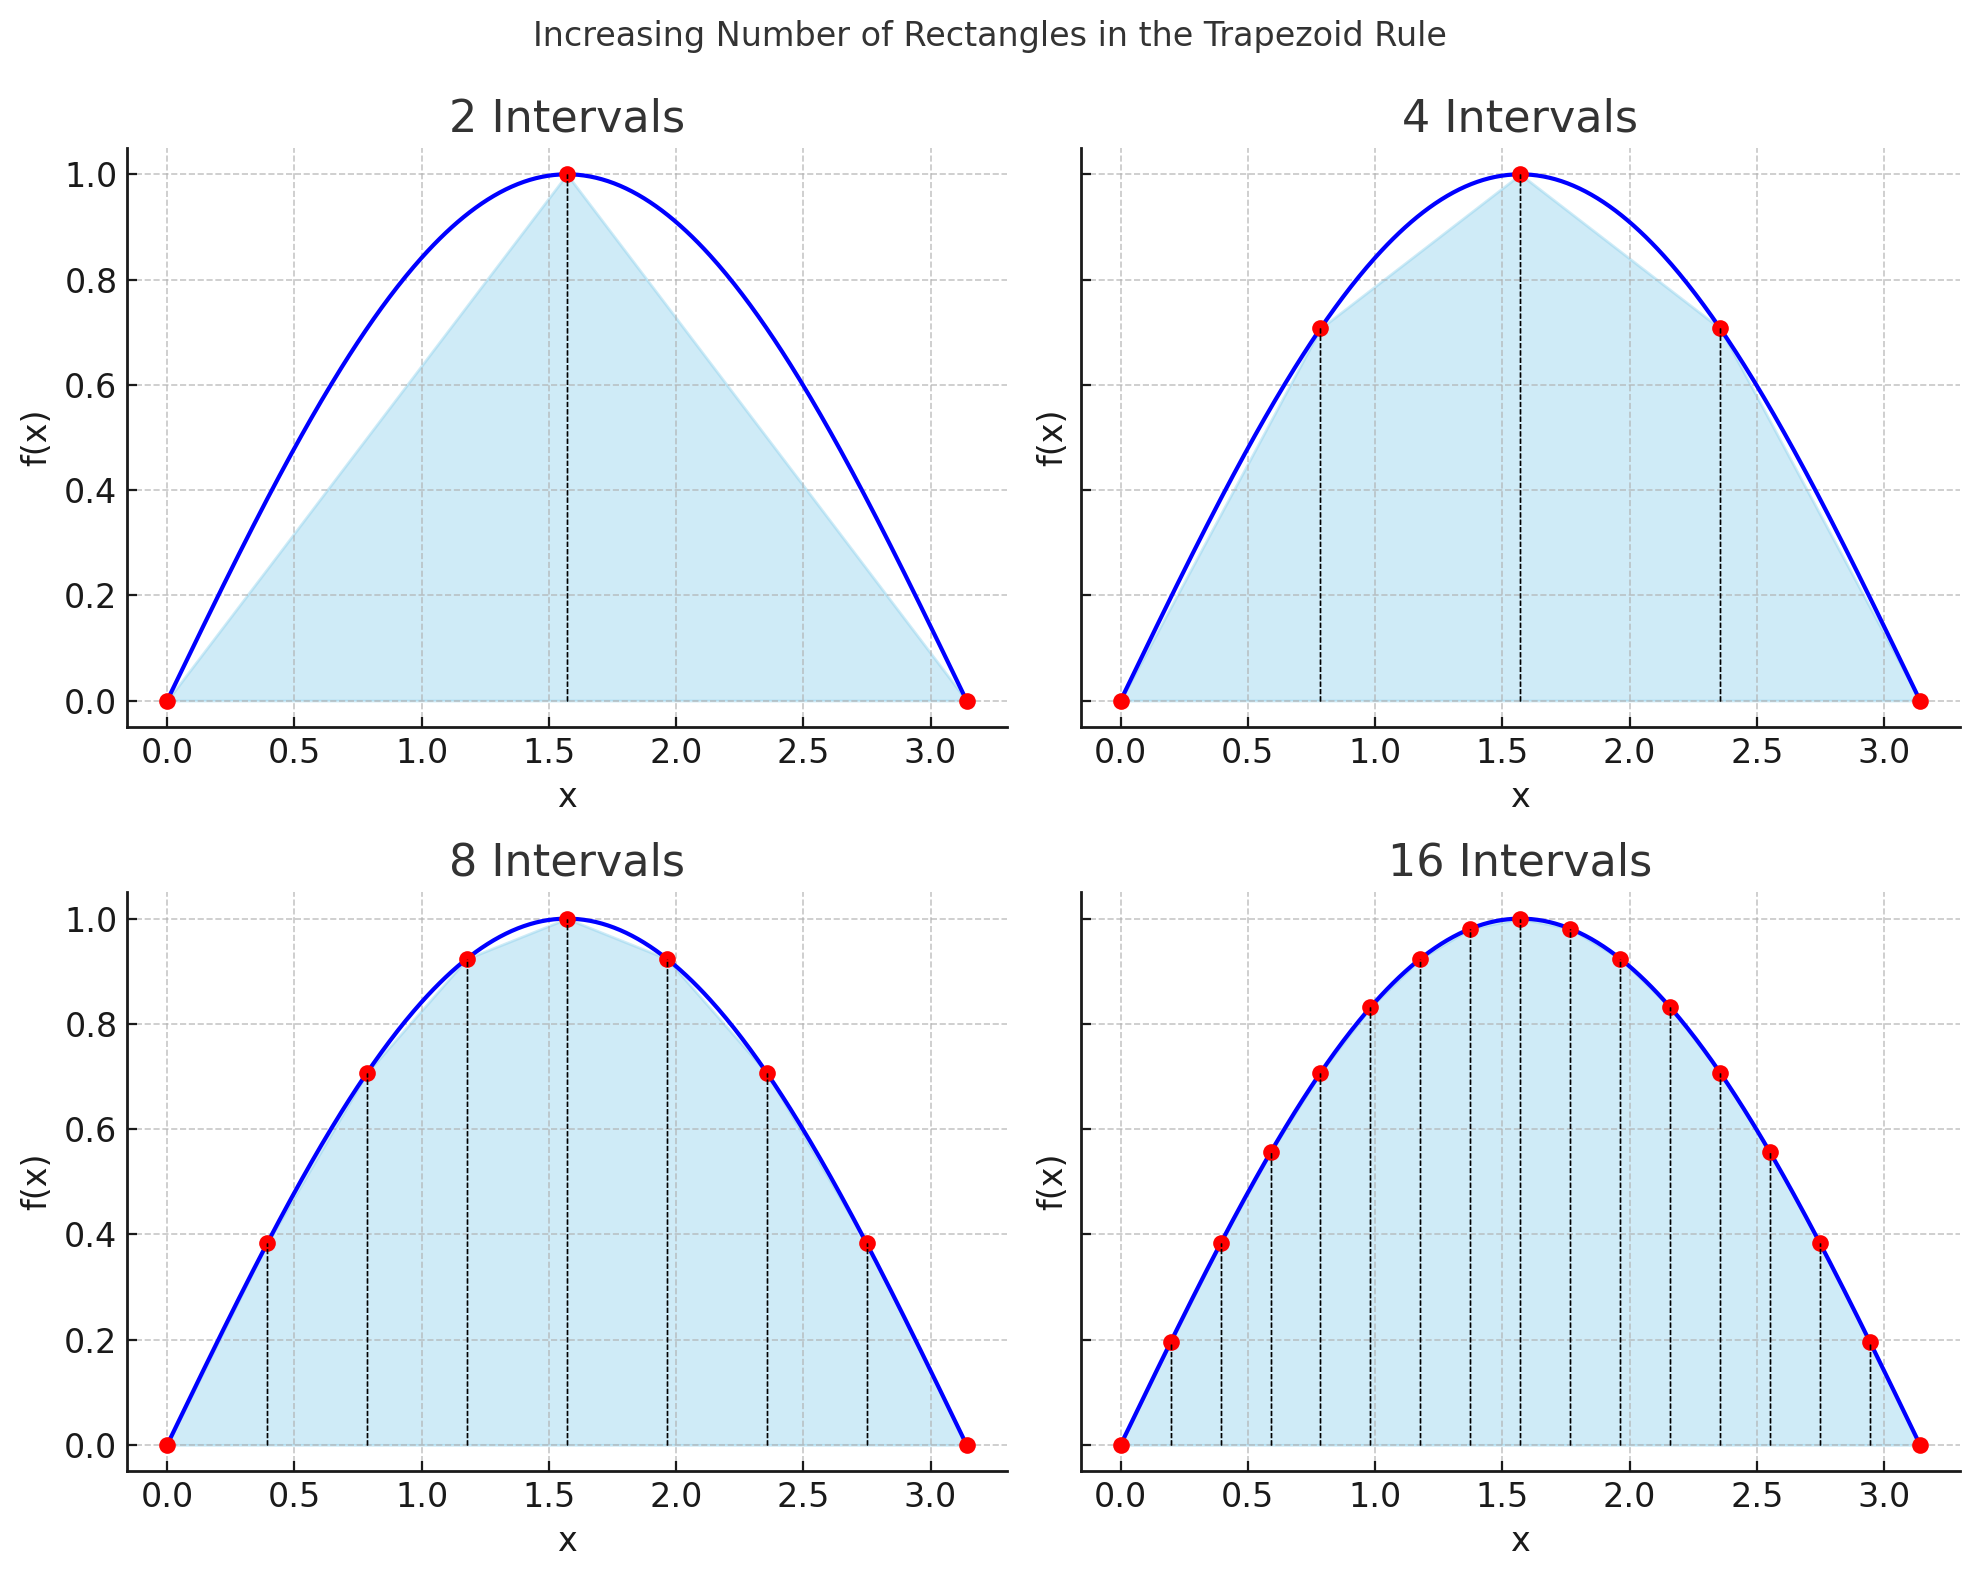
\includegraphics[width=0.75\textwidth]{examples/fig/trap.png}
    \end{center}
\end{frame}
\begin{frame}
  \frametitle{Scipy \texttt{scipy.integrate.trapezoid}}
  \lstinputlisting[language=python]{examples/trapezoid_example.py}
\end{frame}
\begin{frame}
  \frametitle{Self-written Trapezoid Rule}
  An implementation of the trapezoid rule from scratch.\\
  You have to do that in one of the exercises.\\ 
    \vspace{5mm}
  Translate the intuition / formula into maybe a loop or do it entierly vectorized.
\end{frame}
\begin{frame}
  \frametitle{Scipy \texttt{scipy.integrate.simpson}}
  The \texttt{scipy.integrate.simpson} function computes the Simpson's rule to approximate the integral.
  \hrefu{https://docs.scipy.org/doc/scipy/reference/generated/scipy.integrate.simpson.html}{\texttt{scipy.simpson}}
    \vspace{5mm}
    Another way to approximate the integral is using Simpson's rule:
    \begin{align*}
        \int_{a}^{b} f(x) \, dx \approx \frac{b - a}{6} \left( f(a) + 4f\left(\frac{a+b}{2}\right) + f(b) \right)
    \end{align*}
    Quadratic interpolation is used to approximate the function between the points \( a \) and \( b \).
\end{frame}
\begin{frame}
    \frametitle{Simpson rule intuition}
    \vspace{-5mm}
    \begin{center}
        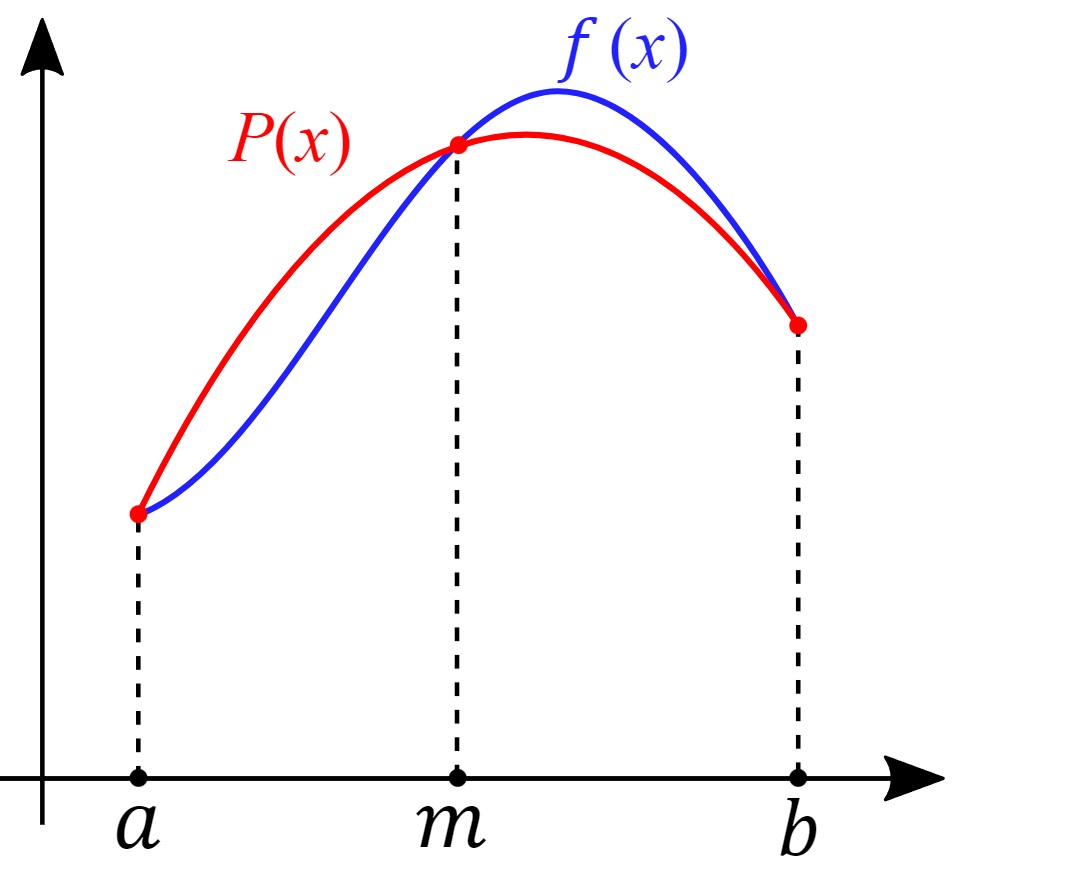
\includegraphics[width=0.75\textwidth]{examples/fig/simpson.png}
    \end{center}
    

\end{frame}
\begin{frame}
  \frametitle{Scipy \texttt{scipy.integrate.simpson}}
  \lstinputlisting[language=python]{examples/simpson_example.py}
\end{frame}

\section{Numerical Solution of Initial Value Problems}

\begin{frame}
  \frametitle{Mathematical Introduction}
  For initial value problems, we discretize the time using $t_n = t_0 + n \Delta t$ and introduce the notation $y_n = y(t_n)$. Thus, we write
  \begin{align*}
    \dot{y}_n &= f(t_n, y_n) \\
    y_{n + 1} &= y_n + \int_{t_n}^{t_{n+1}}dt' f(t', y(t'))
  \end{align*}
  which is still exact. We can now approximate the integral in various ways.
\end{frame}

\begin{frame}
  \frametitle{Explicit Euler Method}
  The explicit Euler method is the simplest method for numerically solving initial value problems. It uses a simple forward difference to approximate the next solution:
  \begin{align*}
    y_{n + 1} &= y_n + \Delta t \cdot f(t_n, y_n)
  \end{align*}
  \begin{itemize}
    \item \textbf{Intuition:} We take a small step $\Delta t$ along the tangent to the solution curve.
    \item \textbf{Accuracy:} This method is only accurate for small $\Delta t$, as it does not account for the curvature of the solution curve.
  \end{itemize}
\end{frame}
\begin{frame}
    \frametitle{Explicit Euler Method intuition }
    \vspace{-5mm}
    \begin{center}
        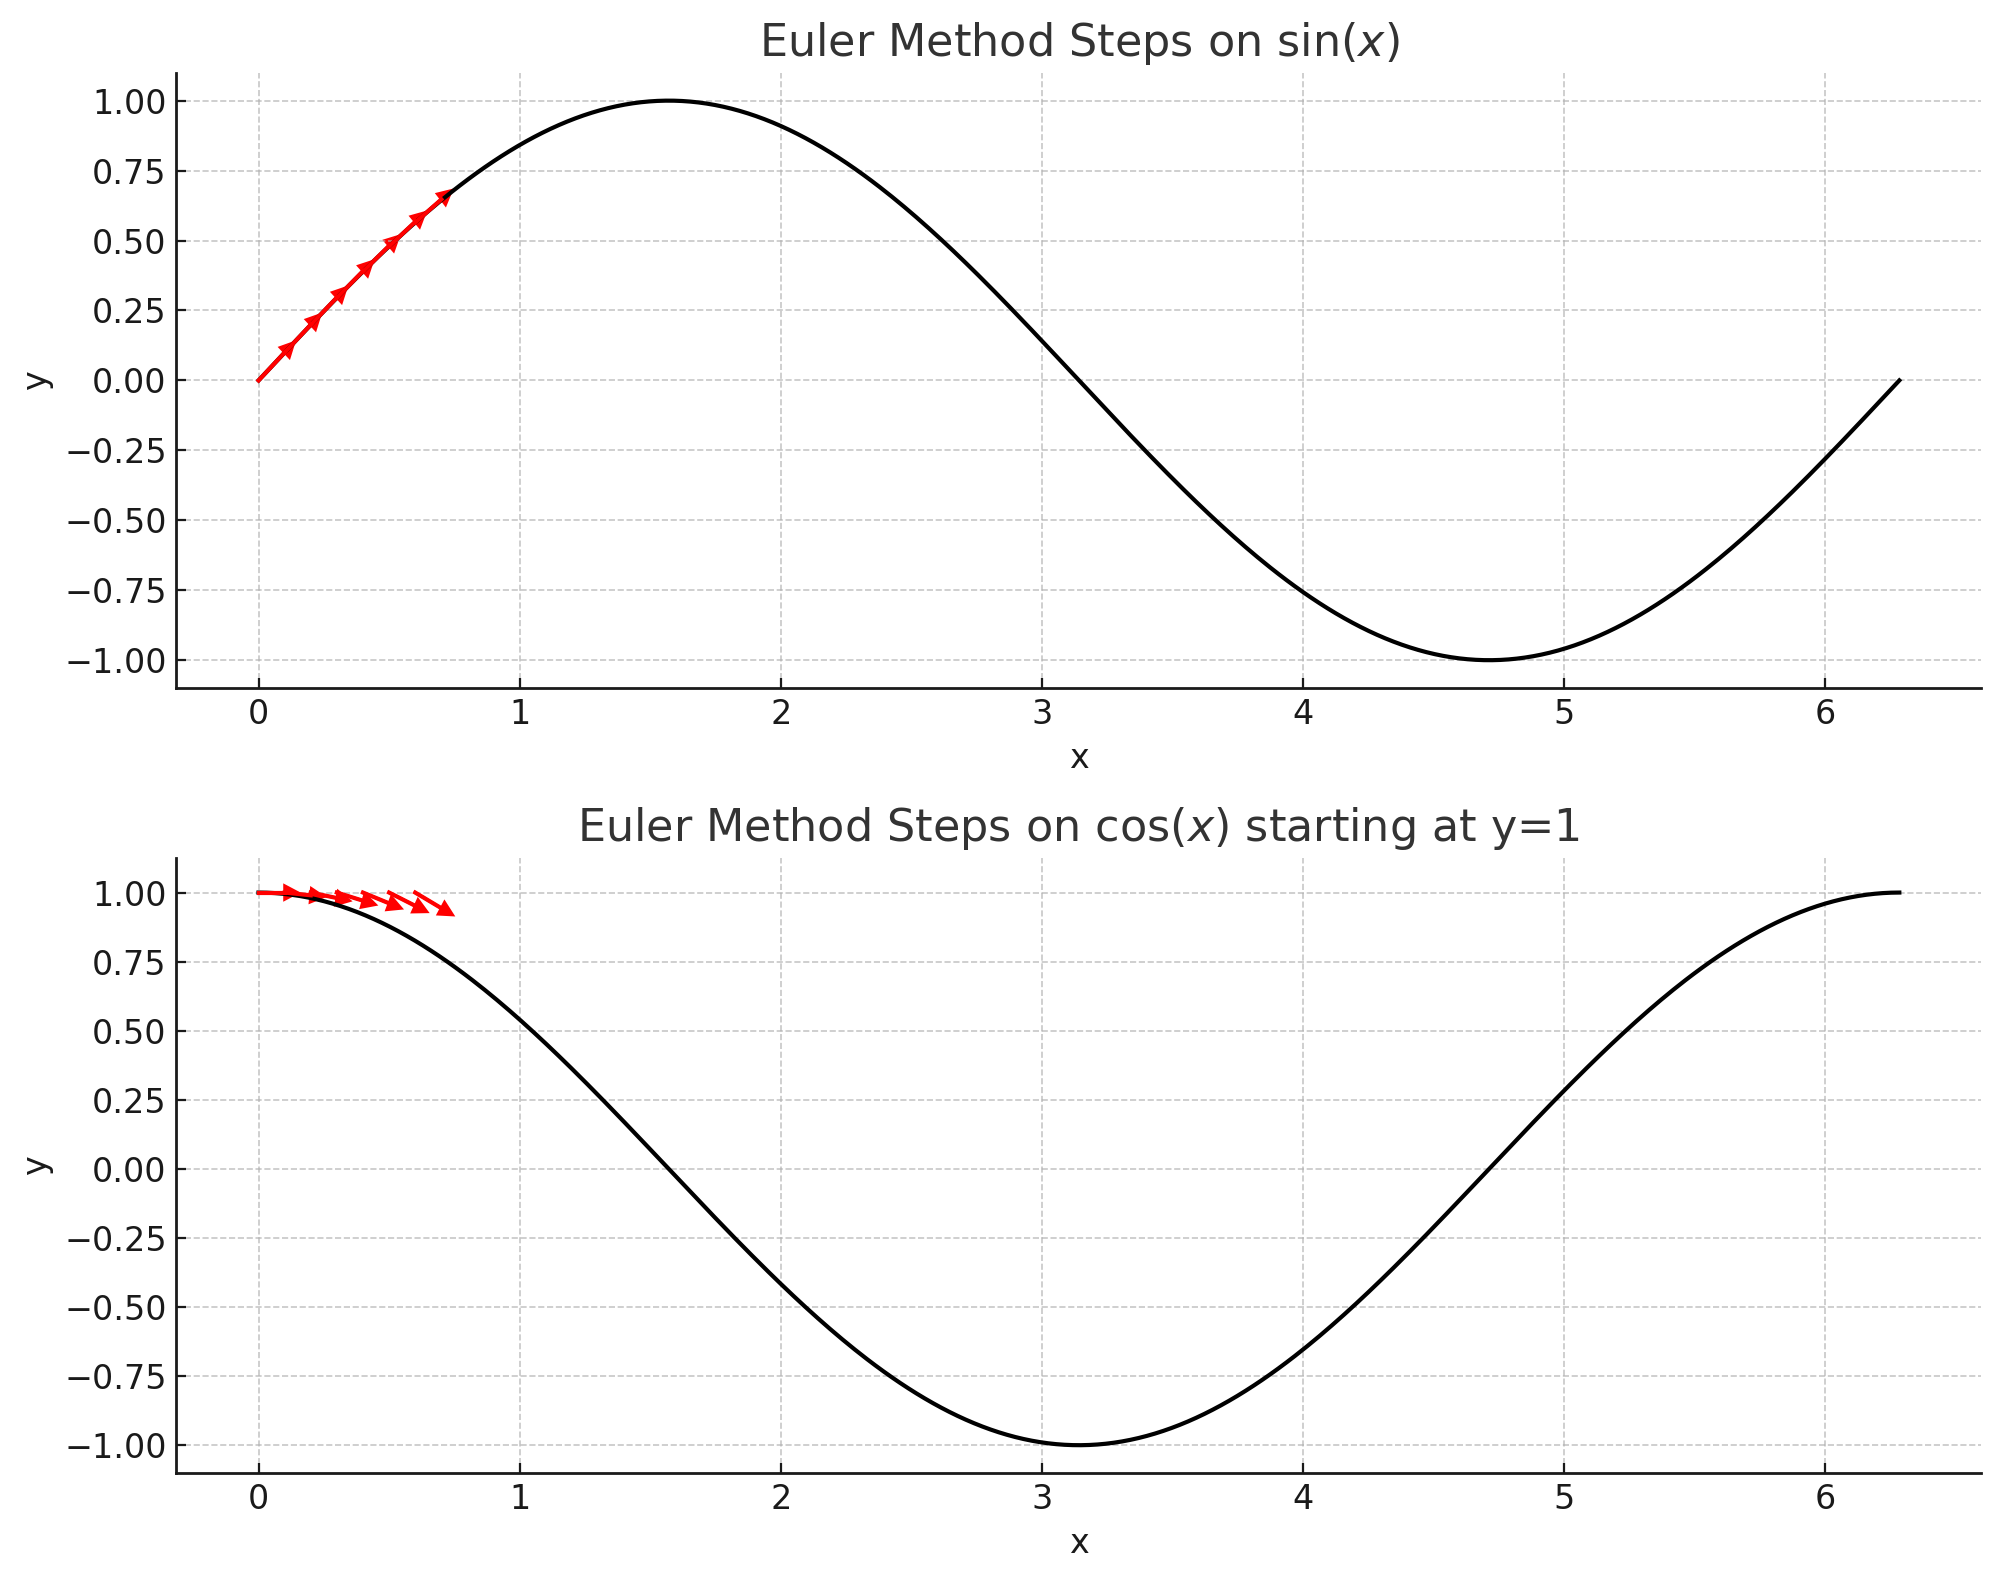
\includegraphics[width=0.75\textwidth]{examples/fig/euler.png}
    \end{center}
\end{frame}
\begin{frame}
    \frametitle{Problems with the Explicit Euler Method}
    As can be seen in the figure on the last slide the explicit Euler method can lead to large errors.\\
    \vspace{5mm}
    Given a start at an extreme point of the function, the values will stay put due to the tangent being parallel to the x-axis: 
    \begin{align*}
        y_{n + 1} &= y_n + \Delta t \cdot f(t_n, y_n) = y_n
    \end{align*}
    because the derivative $ f(t_n, y_n) = 0 $.
\end{frame}

\begin{frame}
  \frametitle{Midpoint Method}
  The midpoint method improves accuracy by using the derivative at the midpoint of the interval:
  \begin{align*}
    y_{n + 1} &= y_n + \Delta t \cdot f\left(t_n + \frac{\Delta t}{2}, y_n + \frac{\Delta t}{2} \cdot f(t_n, y_n)\right)
  \end{align*}
  \begin{itemize}
    \item \textbf{Intuition:} We first compute a preliminary value at the midpoint of the interval and then use this value to calculate the next step.
    \item \textbf{Accuracy:} Higher than the explicit Euler method, as it better accounts for the curvature.
  \end{itemize}
\end{frame}
\begin{frame}
    \frametitle{Midpoint Method intuition}
    \vspace{-5mm}
    \begin{center}
        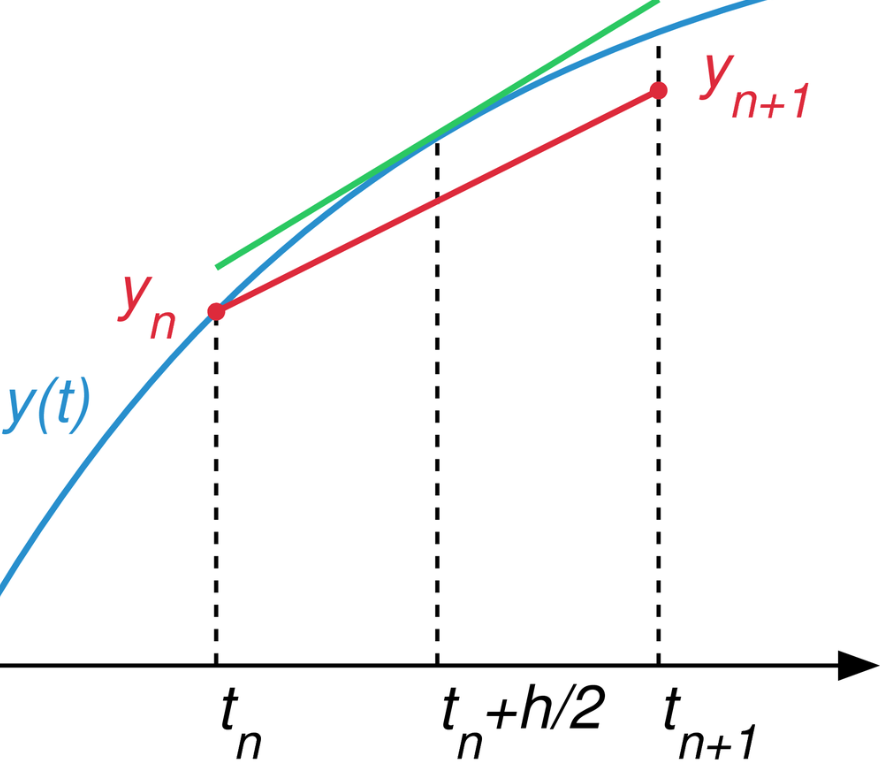
\includegraphics[width=0.6\textwidth]{examples/fig/midpoint2.png}
    \end{center}
\end{frame}
\begin{frame}
    \frametitle{Midpoint Method intuition}
    \vspace{-5mm}
    \begin{center}
        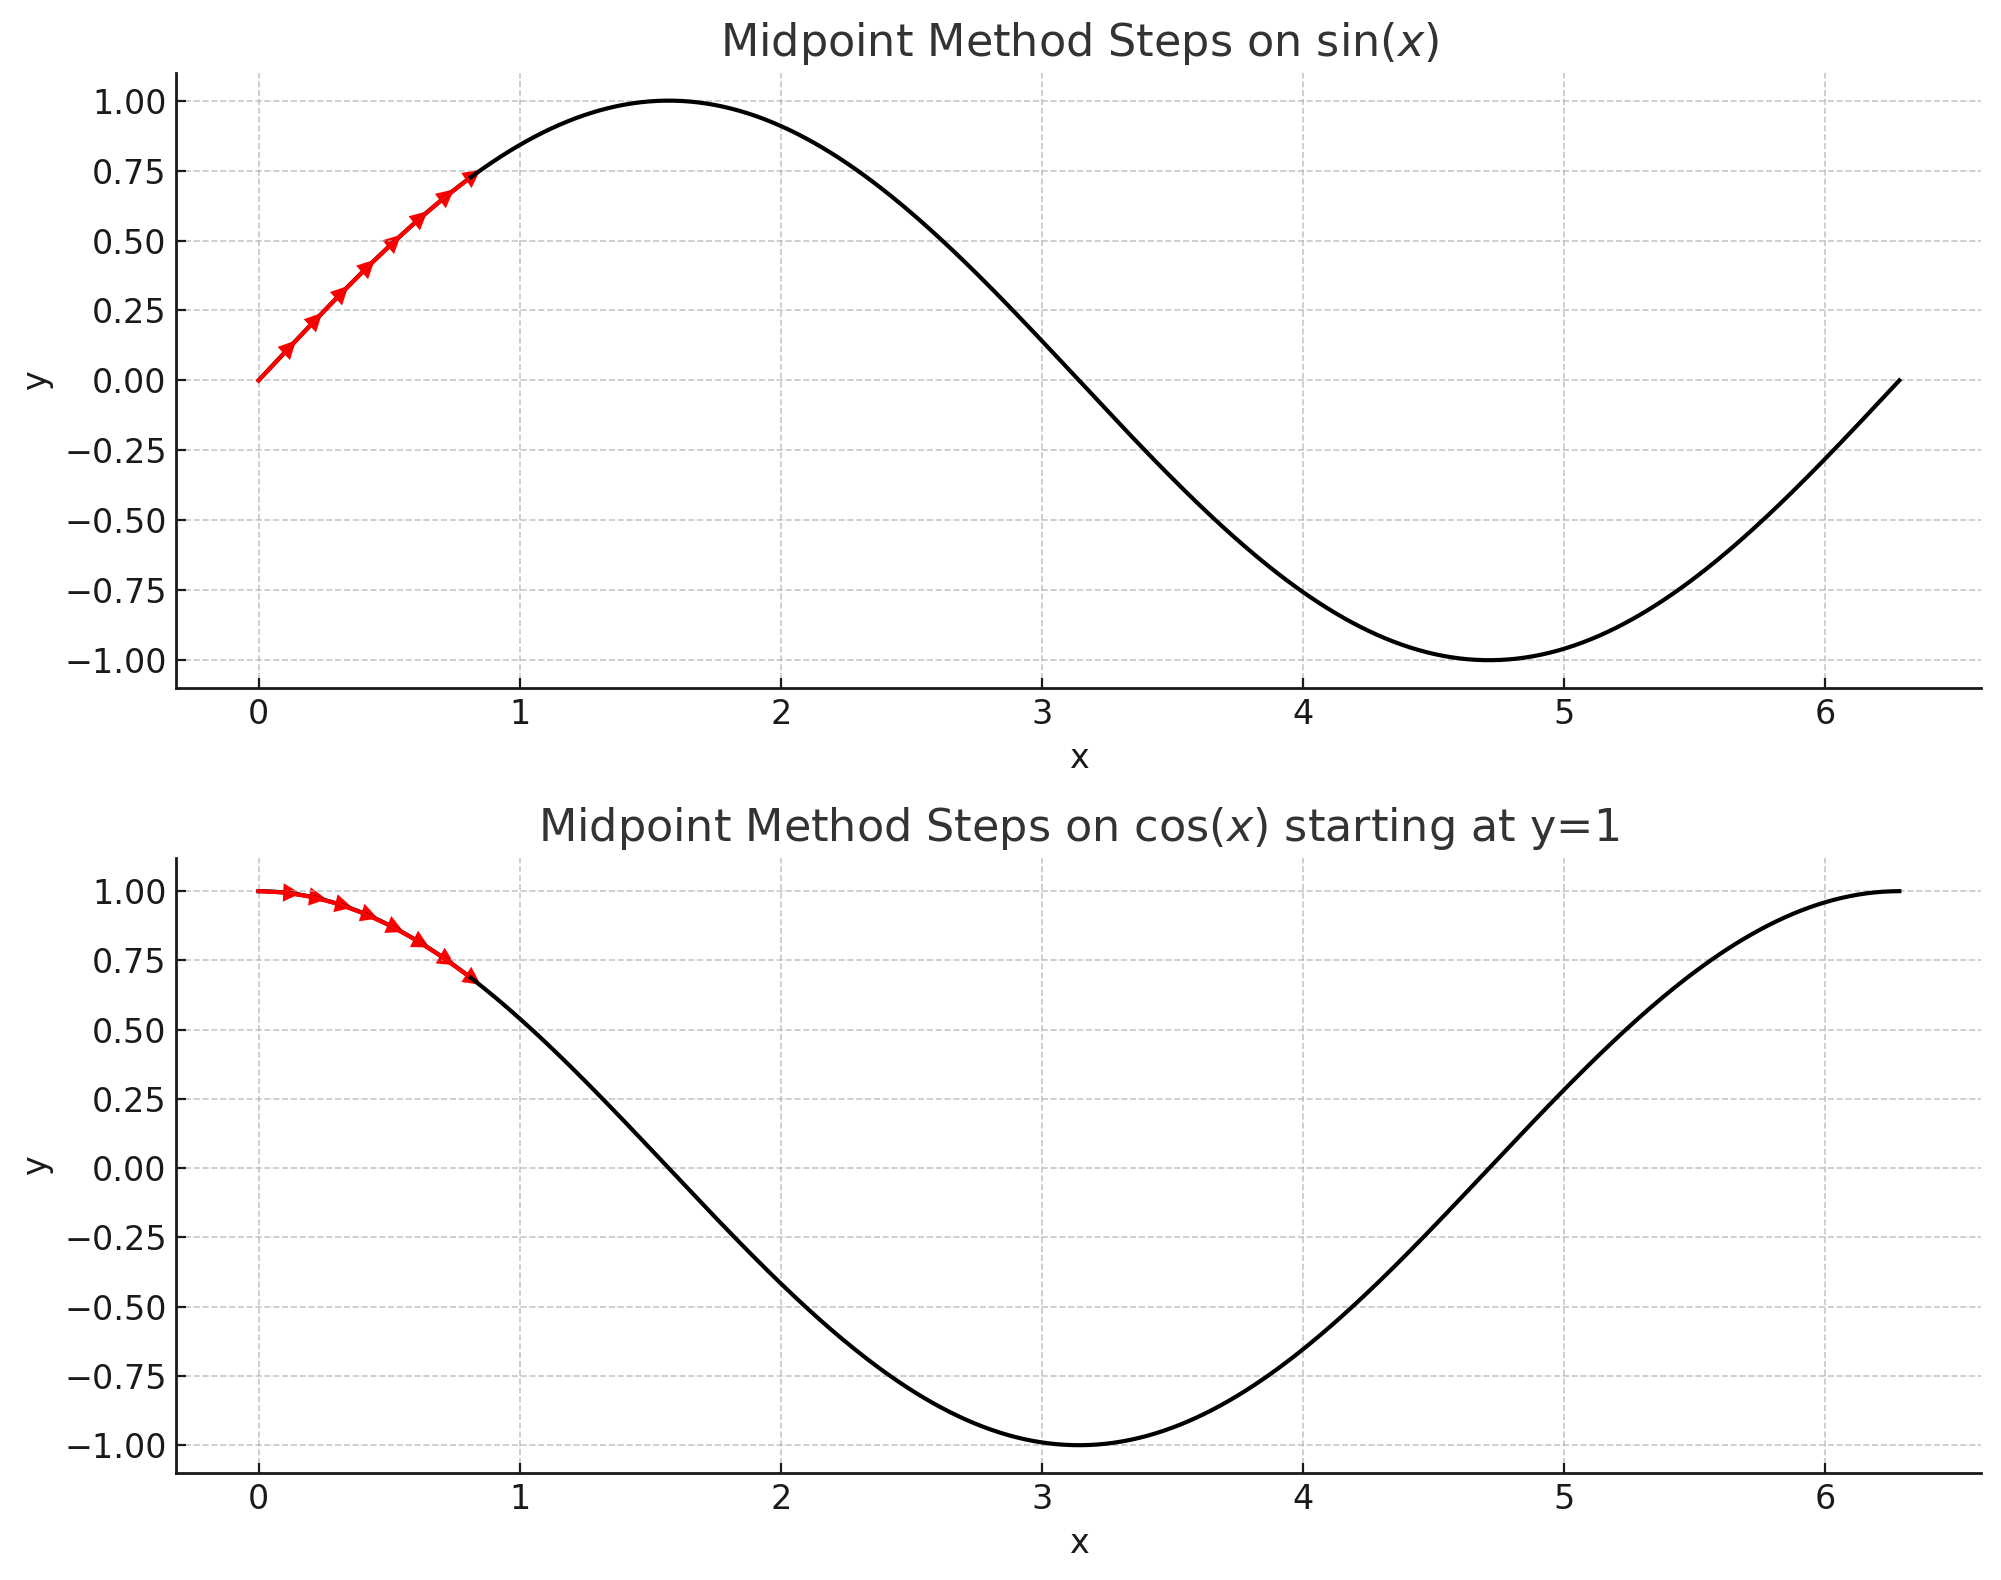
\includegraphics[width=0.75\textwidth]{examples/fig/midpoint.png}
    \end{center}
\end{frame}
\begin{frame}
    \frametitle{Improvement of the Midpoint Method over the Explicit Euler Method}
    Even if the derivative is zero: $ f(t_n, y_n) = 0 $, the midpoint method will still take a step.\\
    \vspace{5mm}
    \begin{align*}
        y_{n + 1} &= y_n + \Delta t \cdot f\left(t_n + \frac{\Delta t}{2}, y_n + \frac{\Delta t}{2} \cdot f(t_n, y_n)\right) \\
        &= y_n + \Delta t \cdot f\left(t_n + \frac{\Delta t}{2}, y_n\right) \\
        &= y_n + \Delta t \cdot f\left(t_n + \frac{\Delta t}{2}, y_n\right) \neq y_n
    \end{align*}
\end{frame}




\section{File I/O (BONUS)}
\begin{frame}
  \frametitle{File I/O -- Basics}
  Python uses \hrefu{https://docs.python.org/3/reference/compound_stmts.html\#with}{with} statements to open and close files.\\
  \lstinputlisting[language=python]{examples/fileio1.py}
\end{frame}
\begin{frame}
  \frametitle{File I/O -- file modes}
  The \texttt{open} function can be used to open files in different modes (multiple are possible):\\
  \begin{table}[h]
  \centering
  \begin{tabular}{|c|c|}
  \hline
  \textbf{File Mode} & \textbf{Description} \\ \hline
  \texttt{r} & Read mode \\ \hline
  \texttt{w} & Write mode \\ \hline
  \texttt{x} & Exclusive creation mode \\ \hline
  \texttt{a} & Append mode \\ \hline
  \texttt{b} & Binary mode \\ \hline
  \texttt{t} & Text mode \\ \hline
  \texttt{+} & Read and write mode \\ \hline
  \end{tabular}
  \label{tab:file-modes}
  \end{table}
\end{frame}

\begin{frame} \frametitle{File I/O -- Reading Files} To read the contents of a file, you can use the \texttt{\hrefu{https://docs.python.org/3/tutorial/inputoutput.html\#methods-of-file-objects}{read()}} method of the file object. This method reads the entire contents of the file and returns it as a string.

  \lstinputlisting[language=python]{examples/fileio2.py}
  
  In this example, we open the file \texttt{input.txt} in read mode (\texttt{r}), read its contents using the \texttt{\hrefu{https://docs.python.org/3/tutorial/inputoutput.html\#methods-of-file-objects}{read()}}  method, and print the contents to the console. \end{frame}
  
  \begin{frame} \frametitle{File I/O -- Writing Files} To write to a file, you can use the \texttt{\hrefu{https://docs.python.org/3/tutorial/inputoutput.html\#methods-of-file-objects}{write()}} method of the file object. This method writes the specified string to the file.
  
  \lstinputlisting[language=python, lastline=3]{examples/fileio3.py}
  
  In this example, we open the file \texttt{example.txt} in write mode (\texttt{w}), write some strings to the file using the \texttt{\hrefu{https://docs.python.org/3/tutorial/inputoutput.html\#methods-of-file-objects}{write()}} method. 
\end{frame}
\begin{frame}
  \frametitle{File I/O -- Reading multiple lines}
  To read multiple lines from a file, you can use the \texttt{\hrefu{https://docs.python.org/3/tutorial/inputoutput.html\#methods-of-file-objects}{readlines()}} method of the file object. This method reads the entire contents of the file, and returns each line as an item in a list.
  \lstinputlisting[language=python, firstline=4]{examples/fileio3.py}
  You do not need to close the file when using the \texttt{with} statement. It is automatically closed when the \texttt{with} block is exited.
\end{frame}

\begin{frame}
  \frametitle{File I/O -- Binary files}
  To read or write binary files, you can use the \texttt{\hrefu{https://docs.python.org/3/tutorial/inputoutput.html\#methods-of-file-objects}{rb}} and \texttt{\hrefu{https://docs.python.org/3/tutorial/inputoutput.html\#methods-of-file-objects}{wb}} modes, respectively:
  \lstinputlisting[language=python, firstline=3]{examples/fileio4.py}
  But how do I know what is in there \dots ?
\end{frame}
\begin{frame}
  \frametitle{File I/O -- Encoding}
  There are many \hrefu{https://en.wikipedia.org/wiki/Character_encoding}{encodings} for text files.\\
  \begin{itemize}
    \item ASCII: 7-bit encoding, 128 characters
    \item Unicode: 16-bit encoding, 65536 characters
    \item UTF-8: 8-bit encoding, variable length, ASCII compatible
    \item ISO-8859-1: 8-bit encoding, 256 characters (Latin-1)
  \end{itemize}
  To interpret a file in the right way, you have to specify the encoding.\\
\end{frame}
\begin{frame}
  \frametitle{File I/O -- Encoding}
  Specify the encoding when opening the file using the \texttt{encoding} argument:
  \lstinputlisting[language=python]{examples/fileio5.py}
  This will fail! Why? 
\end{frame}
\begin{frame}
  \frametitle{File I/O -- Encoding}
  The specified encoding has to match the encoding of the file!\\
  \vspace{5mm}
  The file was written using \texttt{UTF-8} encoding and later read using \texttt{ASCII} encoding which is doomed to fail, since an \glq Ö\grq is in the textfile.\\
  \begin{center}
    \includegraphics[width=\textwidth]{examples/fig/ascii\_fail.png}
  \end{center}
\end{frame}
\section{ASCII Encoding (BONUS)}
\begin{frame}
  \frametitle{ASCII - Table}
    \hrefu{https://de.wikipedia.org/wiki/American_Standard_Code_for_Information_Interchange}{ASCII} (American Standard Code for Information Interchange) is a character encoding standard that assigns unique numeric codes to each character in the English alphabet, as well as various punctuation marks and other symbols.
\end{frame}
\begin{frame}
  \frametitle{ASCII - Table}
  \begin{center}
    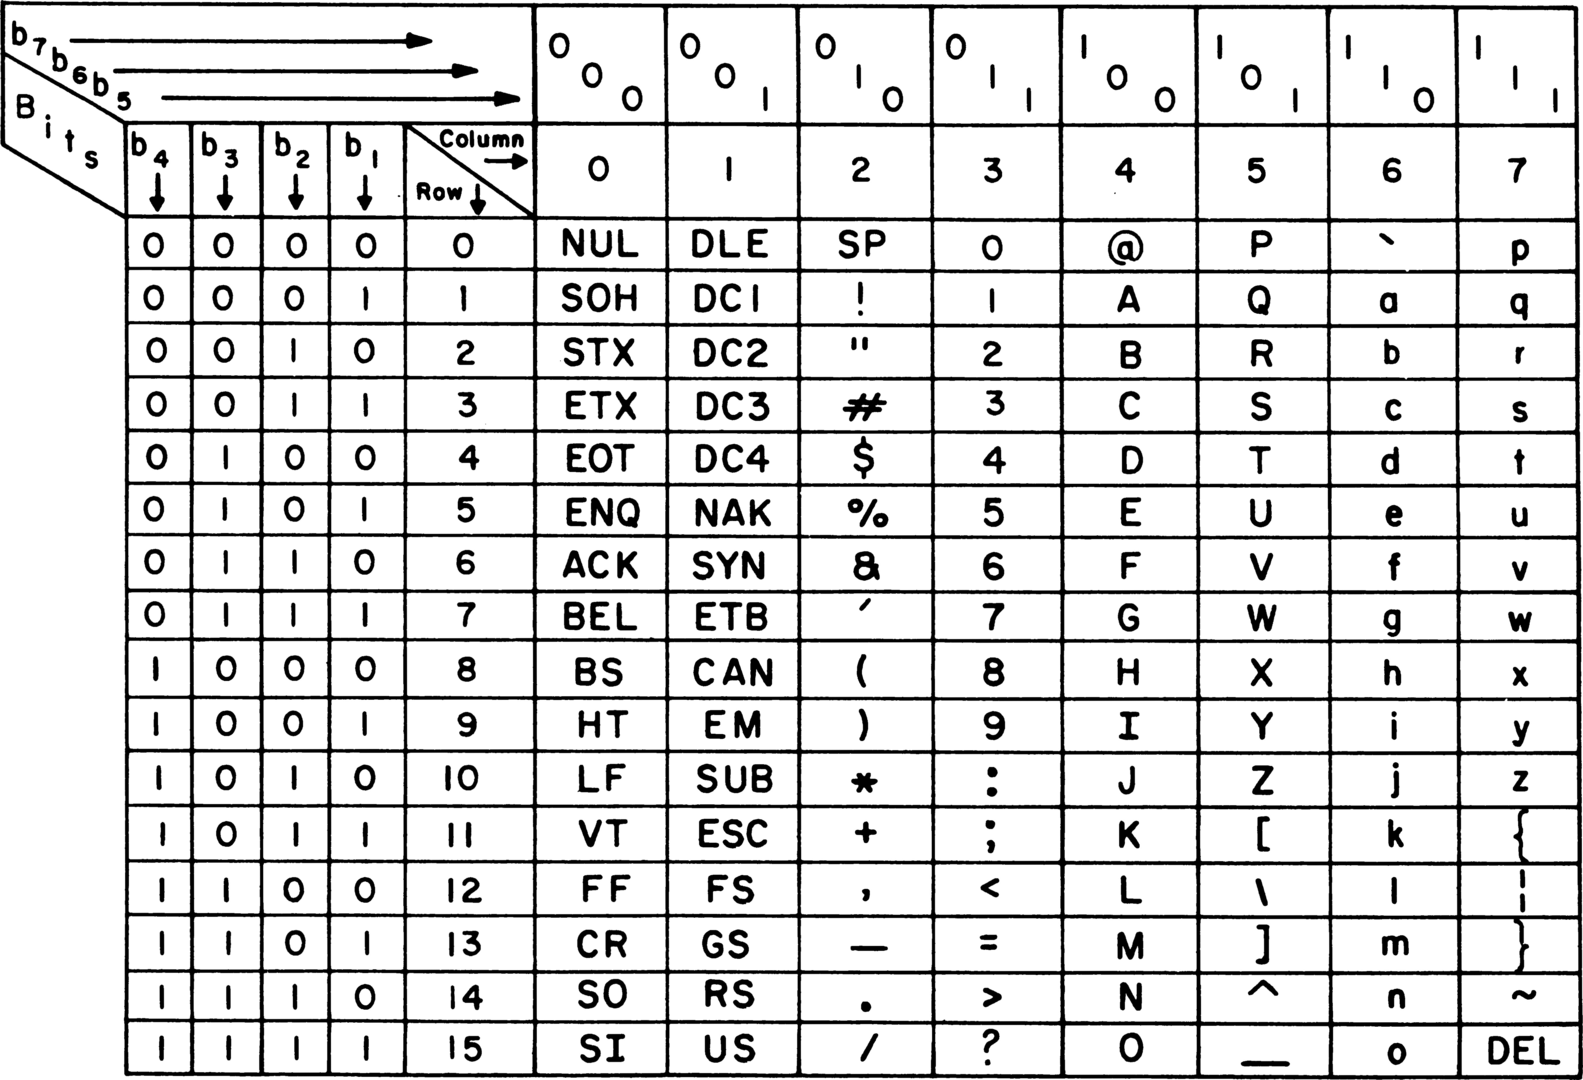
\includegraphics[width=0.75\textwidth]{examples/fig/ASCII.png}
  \end{center}
  \begin{flushleft}
    \vspace{-4mm}
    \tiny\url{https://de.wikipedia.org/wiki/American\_Standard\_Code\_for\_Information\_Interchange\#/media/Datei:USASCII\_code\_chart.png}
  \end{flushleft}
\end{frame}
\begin{frame}
  \frametitle{ASCII - Table}
  This way everything is up to interpretation: 
  You can read the file as ASCII if there are no special characters in it.:
  \lstinputlisting[language=python, lastline=5]{examples/ascii.py}
\end{frame}
\begin{frame}
  \frametitle{Using other encodings}
  With another encoding you can read special characters such as \glq Ö\grq:
  \lstinputlisting[language=python, firstline=6]{examples/ascii.py}
\end{frame}
\section{pickle (BONUS)}
\begin{frame}
  \frametitle{pickle}
  \texttt{\hrefu{https://docs.python.org/3/library/pickle.html}{pickle}} is a module that allows you to store almost any Python object (lists, dictionaries, \dots) in a file.\\
  \vspace{5mm}
  \texttt{\hrefu{https://docs.python.org/3/library/pickle.html}{pickle}} is a binary format, so you have to open the file in binary mode (\texttt{wb} or \texttt{rb}).\\
  \vspace{5mm}
  Use the \texttt{\hrefu{https://docs.python.org/3/library/pickle.html\#pickle.dump}{dump()}} method to write an object to a file, and the \texttt{\hrefu{https://docs.python.org/3/library/pickle.html\#pickle.load}{load()}} method to read an object from a file.
\end{frame}
\begin{frame}
  \frametitle{pickle -- Example}
  \lstinputlisting[language=python]{examples/pickle\_example.py}
\end{frame}

\end{document}
%%%%%%%%%%%%%%%%%%%%%%%%%%%%%%%%%%%%%%%%%%%%%%%%%%%%%%%%%%%%%%%%%%%%%%%%%%%%

%% EOF
